\documentclass[diploma]{softlab-thesis}

%%%
%%%  Add and configure the packages that you need for your thesis
%%%

\usepackage{minted}
\usepackage{amsmath}
\usepackage{amssymb,longtable}
\usepackage{enumitem}
\usepackage{bm}

\usepackage{tikz}
\usetikzlibrary{calc}
\usetikzlibrary{arrows.meta}
\usetikzlibrary{positioning}
%% I define a "style" for the "cells"
\tikzset{
  my cell/.style={
    draw,
    minimum size=5ex,
    node distance=0pt,
  }}
%% to make changing appearances for various aspects of
%% the diagram easier, I define several macros which need
%% only be changed here.  Even though two of these macros
%% have the same definition, I use two to allow the possibility
%% that these styles could be diffferent.
\newcommand\mynodestyle{\sffamily}
\newcommand\myrelocatestyle{\sffamily\bfseries}
\newcommand\mynumberstyle{\sffamily}
\newcommand*\circled[1]{\tikz[baseline=(char.base)]{
   \node[shape=circle,draw,inner sep=1pt] (char) {#1};}}

\DeclareMathSymbol{\mlq}{\mathord}{operators}{``}
\DeclareMathSymbol{\mrq}{\mathord}{operators}{`'}
%%%
%%%  The document
%%%

\begin{document}

%%%  Title page

\frontmatter

\title{Σχεδίαση και Υλοποίηση μιας Καταπληκτικής Γλώσσας Προγραμματισμού}
\author{Νίκος Μαυρογεώργης}
\authoren{Nikos Mavrogeorgis}
\date{Αύγουστος 2019}
\datedefense{26}{8}{2019}

\supervisor{Νικόλαος Σ. Παπασπύρου}
\supervisorpos{Καθηγητής Ε.Μ.Π.}

\committeeone{Νικόλαος Σ. Παπασπύρου}
\committeeonepos{Καθηγητής Ε.Μ.Π.}
\committeetwo{Πέτρος Παπαδόπουλος}
\committeetwopos{Επίκ. Καθηγητής Ε.Μ.Π.}
\committeethree{Γεώργιος Νικολάου}
\committeethreepos{Αν. Καθηγητής Ε.Κ.Π.Α.}

\TRnumber{CSD-SW-TR-42-17}  % number-year, ask nickie for the number
\department{Τομέας Τεχνολογίας Πληροφορικής και Υπολογιστών}

\maketitle


%%%  Abstract, in Greek

\begin{abstractgr}%
  Σκοπός της παρούσας εργασίας είναι αφενός η σχεδίαση μίας απλής
  γλώσσας υψηλού επιπέδου με υποστήριξη για προγραμματισμό με
  αποδείξεις, αφετέρου η υλοποίηση ενός μεταγλωττιστή για τη γλώσσα
  αυτή που θα παράγει κώδικα για μία γλώσσα ενδιάμεσου επιπέδου
  κατάλληλη για δημιουργία πιστοποιημένων εκτελέσιμων.

\begin{keywordsgr}
  Γλώσσες προγραμματισμού,
  Προγραμματισμός με αποδείξεις,
  Ασφαλείς γλώσσες προγραμματισμού,
  Πιστοποιημένος κώδικας.
\end{keywordsgr}
\end{abstractgr}


%%%  Abstract, in English

\begin{abstracten}%
  The purpose of this diploma dissertation is on one hand the design
  of a simple high-level language that supports programming with
  proofs, and on the other hand the implementation of a compiler for
  this language. This compiler will produce code for an
  intermediate-level language suitable for creating certified
  binaries.

  \begin{keywordsen}
  Programming languages,
  Programming with proofs,
  Secure programming languages,
  Certified code.
\end{keywordsen}
\end{abstracten}


%%%  Acknowledgements

\begin{acknowledgementsgr}
  Ευχαριστώ θερμά τον επιβλέποντα καθηγητή αυτής της διατριβής,
  κ.~Νίκο Παπασπύρου
\end{acknowledgementsgr}

\begin{acknowledgementsen}
  I would like to thank all the people who supported my work and helped me get
  results of better quality.  
\end{acknowledgementsen}


%%%  Various tables

\tableofcontents
%\listoftables
\listoffigures
%\listofalgorithms

%%%  Main part of the book

\mainmatter

\chapter{ Εισαγωγή }

Κάθε γλώσσα προγραμματισμού από τη φάση σχεδιασμού της έχει ακριβείς κανόνες που καθορίζουν τη συντακτική δομή των σωστά διατυπωμένων προγραμμάτων της. \cite{Aho2006}
Στη C, για παράδειγμα, ένα πρόγραμμα αποτελείται από συναρτήσεις, μια συνάρτηση από δηλώσεις και εντολές, μια εντολή από εκφράσεις, και ούτω καθ' εξής.
Πρακτικά όλες οι γλώσσες που χρησιμοποιούνται συχνά σήμερα, τόσο φυσικές γλώσσες όσο και γλώσσες μηχανής, βασίζονται στην έκφραση της πληροφορίας με γραμμικό τρόπο, 
όπως οι ακολουθίες συμβόλων  \cite{Ford2002a}.
Το κείμενο σε μία γραπτή γλώσσα συνήθως αναπαρίσταται ως μία  \textit{ συμβολοσειρά}, δηλαδή μια ακολουθία χαρακτήρων που προέρχονται από ένα τυποποιημένο σύνολο. 
Το πρώτο πράγμα που πρέπει να κάνει οποιαδήποτε εφαρμογή επεξεργασίας γλώσσας, 
είναι να μετατρέψει αυτές τις συμβολοσειρές σε πιο αφηρημένες δομές όπως λέξεις, φράσεις, προτάσεις, εκφράσεις ή εντολές.
Η διαδικασία που εξάγει τέτοια χρήσιμη δομημένη πληροφορία από γραμμικό κείμενο είναι γνωστή ως συντακτική ανάλυση ή parsing.

\section{ Ορισμός συντακτικού}

Προκειμένου να κατασκευάσουμε έναν συντακτικό αναλυτή (ή  parser) για μία γλώσσα, ή ακόμα και για να ορίσουμε τυπικά ποια είδη συμβολοσειρών έχουν νόημα σε αυτήν, πρέπει να έχουμε έναν τρόπο να για να εκφράσουμε και να κατανοήσουμε τη συντακτική δομή της.
Για το σκοπό αυτό συνήθως χρησιμοποιούμε κάποια  \textit{ γραμματική}, που είναι μία συμπαγής αναπαράστησαση της δομής μίας γλωσσας, εκφρασμένη σε κάποια άλλη (ιδανικά μικρή και απλή) γλώσσα.
Η γλώσσα της οποίας της δομή προσπαθούμε να αναπαραστήσουμε είναι η  \textit{ γλώσσα αντικείμενο}, ενώ η γλώσσα στην οποία \textit{ εκφράζεται} η συντακτική δομή ονομάζεται  \textit{γραμματική ορισμού γλώσσας}. 

Ο πιο συνηθισμένος τύπος γραμματικής σήμερα, είναι οι \textit{γραμμτικές χωρίς συμφραζόμενα ( context-free grammars - CFG)}, εκφρασμένες σε  Backus-Naur Form (BNF). 
Μία γραμματική χωρίς συμφραζόμενα ουσιαστικά εκφράζει ένα σύνολο αμοιβαίως αναδρομικών κανόνων, οι οποίες περιγράφουν πώς μπορουυν να γραφτούν οι συμβολοσειρές που περιγράφονται στη γλώσσα.
Κάθε κανόνας ή \textit{ παραγωγή}  σε μία  CFG καθορίζει έναν τρόπο με τον οποίο μία συντακτική μεταβλητή ή  \textit{ μη τερματικό} μπορεί να αντικατασταθεί σε μία συμβολοσειρά. 
Ένα μη τερματικό μπορεί να αντικατασταθείξλ σε μία συμβολοσειρά που μπορεί να περιέχει άλλα μη τερματικά, τα οποία θα αντικατασταθούν με τη σειρά τους, ώσπου να μην υπάρχουν άλλα.
Επειδή υπάρχουν πολλοί τρόποι για να αντικατασταθεί ένα μη τερματικό, η γραμματική μπορεί να εκφράσει ένα άπειρο σύνολο καλώς ορισμένων συμβολοσειρών.
Η συντακτική ανάλυση μιας συμβολοσειράς, της οποίας η σύνταξη περιγράφεται από μία  CFG, περιλαμβάνει την ανάποδη διαδικασία: 
να καθοριστεί από μία πλήρως ανεπτυγμένη συμβολοσειρά, η οποία περιέχει μόνο ατομικούς χαρακτήρες ή  \textit{ τερματικά}, ποια ακολουθία (ή ακολουθίες βημάτων) αντικατάστασης, αν υπάρχουν, οδηγούν στην παραγωγή της συμβολοσειράς.
Αυτή η εργασία περιπλέκεται καθώς οι  CFGs  συνήθως περιέχουν αμφισημίες:
σε  \textit{τοπικό επίπεδο}, όπου η σωστή ερμηνεία ενός τμήματος της συμβολοσειράς μπορεί να καθοριστεί μόνο από τα συμφραζόμενα; 
σε \textit{καθολικό επίπεδο}, όπου ολόκληρη η συμβολοσειρά μπορεί να έχει πολλαπλές έγκυρες συντακτικές ερμηνείες.

\section{ Parsing Expression Grammars}
 Η θεωρία και η πράξη της συντακτικής ανάλυσης βασίζεται σε \textit{ παραγωγικά ( generative)} συστήματα, όπως οι κανονικές εκφράσεις και οι γραμματικές χωρίς συμφραζόμενα, στα οποία η γλώσσα ορίζεται τυπικά μέσα από κανόνες οι οποίοι όταν εφαρμοστούν αναδρομικά παράγουν συμβολοσειρές της γλώσσας.
Αντίθετα, σε ένα \textit{ αναγνωριστικό σύστημα ( recognition-based system)} η γλώσσα ορίζεται μέσα από κανόνες ή κατηγορήματα που αποφασίζουν εάν η δοθείσα συμβολοσειρά ανήκει στη γλώσσα \cite{Ford2004}.
Οι απλές γλώσσες μπορούν να εκφραστούν εξίσου εύκολα και στα δύο συστήματα.
 Για παράδειγμα, το $\{ s \in \mathbf{a}^* | s = {(\mathbf{a}\mathbf{a})}^n\}$ είναι ένας παραγωγικός ορισμός μιας γλώσσας με ένα μόνο γράμμα στο λεξιλόγιό της, της οποίας οι συμβολοσειρές 
 κατασκευάζονται συνενώνοντας ζεύγη από $ \mathbf{a}$.
 Από την άλλη, το $\{ s \in \mathbf{a}^* | (\lvert s \rvert mod2=0)\}$, είναι ένας αναγνωριστικός ορισμός, όπου μία συμβολοσειρά από  $\mathbf{a}$'s γίνεται αποδεκτή μόνο αν το μήκος της είναι άρτιο.
 
  Αν και το παραγωγικό μοντέλο χρησιμοποιείται ευρύτατα στη θεωρία γλωσσών, οι πιο πολλές πρακτικές γλωσσικές εφαρμογές περιλαμβάνουν την αναγνώριση και τη δομική ανάλυση συμβολοσειρών. 
Εμείς θα χρησιμοποιήσουμε το αναγνωριστικό μοντέλο για τη σύνταξη της γλώσσας, η οποία θα περιγράφεται από τις  \textit{Parsing Expression Grammars (PEGs)}. Αυτές μοιάζουν με τις γραμματικές χωρίς συμφραζόμενα με την προσθήκη χαρακτηριστικών από τις κανονικές εκφράσεις, όμοια με την  Extended BNF σημειογραφία.

\section{ Packrat Parsing}
Με βάση τις Parsing Expression Grammars και το αναγνωριστικό σχήμα, ο απλούστερος τρόπος να αναλυθεί (συντακτικά) μία συμβολοσειρά έιναι μέσω ενός αναδρομικού καθοδικού συντακτικού αναλυτή, με δυνατόττηα για οπισθαναχώρηση ( backtracking). 
Ωστόσο, σε πολλές  PEGs  ένας συνήθης καθοδικός αναλυτής μπορεί να κάνει εκθετικό χρόνο για να αναγνωρίσει μία συμβολοσειρά στην είσοδο. 
Και αυτό διότι η οπισθαναώρηση μπορεί να οδηγήσει σε πλεονάζοντες υπολογισμούς ενδιάμεσων αποτελεσμάτων.
Αν, όμως, χρησιμοποιηθεί \textit{ υπομνηματισμός ( memoisation)} για να αποφευχθούν τέτοιοι πλεονασμοί, μία  PEG  μπορεί να αναλυθεί σε γραμμικό χρόνο με το μήκος της εισόδου.
Ένας τέτοιος συντακτικός αναλυτής ονομάζεται \textit{Packrat Parser}.

\section{ Αυτόματη παραγωγή των  Packrat Parsers}
Αν και το  packrat parsing είναι εύκολο να υλοποιηθεί με το χέρι, θα ήταν ακόμη καλύτερο να μπορούσαμε να κατασκευάσουμε τέτοιους συντακτικούς αναλυτές με αυτόματο τρόπο, όμοια με το  YACC  στον κόσμο της C. 
Ένας \textit{γεννήτορας συντακτιών αναλυτών (parser generator)} παίρνει ως είσοδο μία τυπική περιγραφή της γραμματικής και "γεννάει" τον αντίστοιχο συντακτικό αναλυτή  σε  C++.
Η περιγραφή που δέχεται ο δικός μας γεννήτορας βασίζεται στη σημειογραφία των  PEGs. 
Τέλος, παρέχει και τη δυνατότητα να επιστραφεί το συντακτικό δέντρο μετά την ανάλυση, ενώ επεκτείνεται εύκολα ώστε να κρατήσει και άλλες σημασιολογικές τιμές.
Οι βασικές ιδέες για την υλοποίησή του πηγάζουν από πρότερη δουλειά που έχει γίνει σε  Java % TODO: \cite{fowler} \cite{lgi}.

\section{  Παράλληλο Packrat Parsing}
Αφού  υλοποιήσουμε έναν  packrat parser generator σε C++, η βασική συνεισφορά που θέλουμε να κάνουμε στα πλαίσια της διπλωματικής, είναι να εξετάσουμε κατά πόσο και πώς ένας σειριακός packrat parser μπορεί να παραλληλοποιθεί ώστε να τρέχει αποδοτικότερα σε ένα πολυπύρηνο σύστημα με αρχιτεκτονική κοινής μνήμης.
Η πρώτη προσέγγιση που έχει δοκιμαστεί (cite fowler) είναι να χωρίζεται η είσοδος σε κομμάτια και να αναλαμβάνει ένα νήμα να υπολογίσει τα κελιά του συντακτικού αναλυτή που αφορούν το συγκεκριμένο κομμάτι. (% TODO: add more about seith fowler)
H  πρώτη δική μας προσέγγιση ήταν να αντί για υπομνηματισμό, να χρησιμοποιήσουμε δυναμικό προγραμματισμό, τον οποίο επειτα δοκιμάσαμε να παραλληλοποιήσουμε.
Ακολούθως, εφαρμόσαμε παραλληλοποίηση στην πράξη της \textit{ επιλογής ( choice)} των  PEGs % TODO: add more about pht
Τέλος, αφού υλοποιήσαμε το  Elastic % TODO: 

\section{  Η δομή της εργασίας}

\chapter{ Parsing Expression Grammars }

Οι δύο πιο συνηθισμένες μέθοδοι για να περιγραφεί η σύνταξη μίας γλώσσας σήμερα είναι οι κανονικές εκφράσεις και οι γραμματικές χωρίς συμφραζόμενα. 
Αυτοί οι φορμαλισμοί, ωστόσο, δεν είναι σε καμία περίπτωση ο μοναδικός τρόπος ορισμούς της συντακτικής δομής μίας γλώσσας. 
Ένα ακόμη χρήσιμο πρότυπο περιγραφής της σύνταξης είναι οι  \textit{Parsing Expression Grammars (PEGs)} \cite{Ford2004}, οι οποίες μοιάζουν με τις γραμματικές χωρίς συμφραζόμενα, αλλά έχουν και ορισμένες θεμελιώδεις διαφορές. 
Δαισθητικά, μια γραμματική χωρίς συμφραζόμενα μας περιγράφει το πώς  \textit{κατασκευάζεται} μία συμβολοσειρά που ανήκει σε κάποια γλώσσα, ενώ οι  PEGs  το πώς  \textit{αναλύεται} η συμβολοσειρά ώστε να προκύψει δομική πληροφορία για αυτή - εξ ου και το όνομα  "parsing language". 

Δεδομένου ότι η περιγραφή των γλωσσών (συνήθως) γράφεται από ανθρώπους και διαβάζεται από μηχανές, οι  Parsing Expression Grammars αποτελούν διαισθητικά ένα πιο κατάλληλο εργαλείο προσδιορισμού 
από της γραμματικές χωρίς συμφραζόμενα. 
Ο σχεδιαστής της γραμματικής είναι ευκολότερο να σκέφτεται πώς αναλύεται μία δοσμένη συμβολοσειρά στα συστατικά της, παρά πώς θα γεννηθεί (generated) η συμβολοσειρά μέσα από τους κανόνες της γραμματικής.
% TODO: example to prove aforementioned claim

Πολλά συντακτικά ιδιώματα των σύγχρονων γλωσσών προγραμματισμού εκφράζονται ευκολότερα και πιο "φυσικά" σε  Parsing Expression Grammars. 
Επιπρόσθετα, οι PEGs μπορούν να αναλυθούν συντακτικά σε γραμμικό χρόνο, χρησιμοποιώντας το  Packrat Parsing  που περιγράφεται σε επόμενη ενότητα, την ώρα που μόνο μία συγκεκριμένη υποκλάση των γλωσσών χωρίς συμφραζόμενα μπορεί να αναλυθεί σε γραμμμικό χρόνο.

\section{Ορισμός των  Parsing Expression Grammars}
 Όπως με τις  Context Free,  οι  Parsing Expression Grammars χρησιμοποιούν τόσο τερματικά όσο και μη τερματικά σύμβολα και αποτελούνται από ένα σύνολο κανόνων που παρέχουν ορισμούς για τα μη τερματικά.
Κάθε κανόνας μπορεί να αναφέρεται σε άλλους κανόνες της γραμματικής αναδρομικά. Θα ακολουθήσουμε το συμβολισμό `$ n \leftarrow e $', όπου το $ n$ είναι ένα μη τερματικό και το $e$ είναι μία έκφραση που θα οριστεί ακολούθως. 
Η χρήση του αριστερού βέλους αντί του δεξιού εκφράζει την διασθητική διαφορά στην "ροή της πληροφορίας" που διακρίνει τις  PEGs από τις CFGs. 
Ενώ, οι κανόνες των CFGs εκφράζουν "παραγωγές" από μη τερματικά στις αντίστοιχες εκφράσεις τους, οι κανόνες των  PEGs αναπαριστούν "αφαιρέσεις" από τις εκφράσεις στους αντίστοιχους κανόνες. 
Επιπλέον, οι παραγωγές εκφρασμένες σε CFGs αναπαριστούν πράξεις σε ολόκληρες συμβολοσειρές, ενώ οι αφαιρέσεις σε μία  PEG  αναπαριστά πράξεις σε προθέματα της συμβολοσειράς στην είσοδο.

Σύμφωνα με τον συμβολισμό των  Parsing Expression Grammars, οι εκφράσεις σχηματίζονται ως εξής:

 \begin{description}[font=$\bullet$\scshape\bfseries]

   \item[ Κενή συμβολοσειρά:] 
	 `()' είναι μία έκφραση που υποδηλώνει την άδεια συμβολοσειρά. 
	 Η ερμηνεία της είναι "Μην προσπαθήσεις να διαβάσεις τίποτα: απλά επίστρεψε επιτυχώς χωρίς να καταναλώσεις τίποτα από την είσοδο."

   \item[ Τερματικό:] 
	 Αν το $ \alpha $ είναι ένα τερματικό σύμβολο (π.χ. ένας χαρακτήρας μόνος του), τότε το `$ \alpha$' είναι μία έκφραση της οποίας η ερμηνεία είναι: 
	 "Αν το επόμενο τερματικό στην είσοδο είναι $ \alpha $ τότε κατανάλωσε ένα τερματικό και επίστρεψε επιτυχώς. αλλιώς, απότυχε και μην καταναλώσεις τίποτα."

   \item[ Μη Τερματικό:]
	 Αν το $ A $ είναι ένα μη τερματικό σύμβολο , τότε το  `$ A $' είναι μία έκφραση της οποίας η ερμηνεία είναι:
	 "Προσπάθησε να διαβάσεις την είσοδο με βάση τον κανόνα που αντιστοιχεί στο  $ A $ και επίστρεψε επιτυχώς ή απότυχε αντίστοιχα."

   \item[ Ακολουθία:]
	 Αν $ e_1, e_2, \ldots, e_n $ είναι εκφράσεις, τότε το  `$(e_1 e_2 \ldots e_n)$' είναι μία έκφραση της οποίας η ερμηνεία είναι: 
	 "Πρώτα προσπάθησε να διαβάσεις μία συμβολοσειρά ώστε να επιτύχει η $e_1$. 
	 Αν η $ e_1$ επιτύχει, τότε προσπάθησε να διαβάσεις μία συμβολοσειρά ώστε να επιτύχει η  $e_2$, ξεκινώντας από το σημείο της εισόδου που δεν κατανάλωσε η  $e_1$. 
	 Αν η  $e_2$ επιτύχει τότε συνέχισε με  την  $e_3$ κ.ό.κ μέχρι την  $e_n$.
	 Αν και οι  $n$ εκφράσεις αναγνωριστούν επιτυχώς διαδοχικά, τότε επίστρεψε επιτυχώς και κατανάλωσε όλα τα αντίστοιχα κομμάτια της εισόδου.
	 Αν οποιαδήποτε υποέκφραση αποτύχει, τότε όλη η ακολουθία αποτυγχάνει συνολικά χωρίς να καταναλώσει τίποτα από την είσοδο."

   \item[ Διατεταγμένη Επιλογή] Αν $ e_1, e_2, \ldots, e_n $ είναι εκφράσεις, τότε το `$(e_1 / e_2 / \ldots / e_n)$' είναι μία έκφραση της οποίας η ερμηνεία είναι η εξής: 
	 "Πρώτα προσπάθησε να διαβάσεις μία συμβολοσειρά ώστε να επιτύχει η $e_1$. 
	 Αν αυτό πετύχει τότε η επιλογή επιστρέφει επιτυχώς καταναλώνοντας το αντίστοιχο κομμάτι της εισόδου.
	 Αλλιώς, προσπάθησε με την $e_2$ και την αρχική είσοδο, μετά με την $e_3$, κ.ό.κ, μέχρις ότου να φτάσεις στην $e_n$, σταματώντας στην πρώτη εναλλακτική που θα επιτύχει.
	 Αν καμία από τις $n$ εναλλακτικές δεν πετύχουν, τότε απότυχε χωρίς να καταναλώσεις τίποτα από την είσοδο."
	 Η έκφραση `$(e_1 / e_2)$' μπορεί να διαβαστεί ως "$e_1 \text{ ή αλλιώς } e_2$". 
	 Χρησιμοποιήσαμε το σύμβολο της καθέτου (`$/$') αντί της μπάρας (`$|$'), που χρησιμοποιείται στις γραμματικές χωρίς συμφραζόμενα, 
	 για να τονίσουμε την ουσιώδη διαφορά ότι η επιλογή στις PEGs δεν είναι συμμετρική, αλλά βασίζεται σε προτεραιότητα.

   \item[ Άπληστη Επανάληψη:]
	 Αν το `$e$' είναι μία έκφραση, τότε το `$(e^*)$' είναι μία έκφραση της οποίας η ερμηνεία είναι η εξής:
	 "Εφάρμοσε την έκφραση $e$ επανειλλημένα στην είσοδο, καταναλώνοτας την είσοδο προοδευτικά με κάθε επανάληψη όσο συνεχίζει να επιτυγχάνει.
	 Με την πρώτη αποτυχία, κατανάλωσε όλη την είσοδο που είχε αναγνωριστεί μέχρι τότε και επίστρεψε επιτυχώς.
	 Αν το $e$ δεν πέτυχε ούτε μία φορά, τότε επίστρεψε όπως και να 'χει επιτυχώς χωρίς να καταναλώσεις τίποτα."

   \item[ Άπληστη Θετική Επανάληψη:] %  TODO: check trans 
	 Αν το `$e$' είναι μία έκφραση, τότε το `$(e^+)$' είναι μία έκφραση της οποίας η ερμηνεία είναι η εξής:
	 "Εφάρμοσε την έκφραση $e$ επανειλλημένα στην είσοδο, 
	 και επίστρεψε επιτυχώς καταναλώνοντας όλη την είσοδο που είχε αναγνωριστεί όσο τουλάχιστον ένα στιγμιότυπο της $e$ πετύχαινε.
	 Με την πρώτη αποτυχία, κατανάλωσε όλη την είσοδο που είχε αναγνωριστεί μέχρι τότε και επίστρεψε επιτυχώς.
	 Αν το $e$ δεν πέτυχε ούτε μία φορά, τότε απότυχε χωρίς να καταναλώσεις τίποτα."

   \item[ Προαιρετικό:] 
	 Αν το `$e$' είναι μία έκφραση, τότε το `$(e?)$' είναι μία έκφραση της οποίας η ερμηνεία είναι η εξής:
	 "Προσπάθησε να εφαρμοσεις την έκφραση $e$ στην είσοδο.
	 Αν πετύχεις, τότε κατανάλωσε το αναγνωρισμένο κείμενο και επίστρεψε επιτυχώς.
	 Αν το $e$ αποτύχει, τότε επίστρεψε επιτυχώς όπως και να `χει αλλά μην καταναλώσεις τίποτα από την είσοδο."

   \item[ Ακουλουθείται-Από Κατηγόρημα:]
	 Αν το `$e$' είναι μία έκφραση, τότε το `$\&(e)$' είναι μία έκφραση της οποίας η ερμηνεία είναι η εξής:
	 "Προσπάθησε να εφαρμόσεις την έκφραση $e$ στην είσοδο.
	 Αν πετύχεις με το `$e$', τότε επίστρεψε επιτυχώς με το `$\&(e)$' αλλά μην καταναλώσεις τίποτα από την είσοδο 
	 (δηλαδή επίστρεψε στην θέση της εισόδου που ήσουν πριν εφαρμοστεί το $e$).
	 Αν το $e$ αποτύχει, τότε απότυχε".

   \item[ Δεν-Ακολουθείται-Από Κατηγόρημα:]
	 Αν το `$e$' είναι μία έκφραση, τότε το `$!(e)$' είναι μία έκφραση της οποίας η ερμηνεία είναι η εξής:
	 "Προσπάθησε να εφαρμόσεις την έκφραση $e$ στην είσοδο.
	 Αν πετύχεις με το `$e$', τότε απότυχε με το `$\!(e)$' αλλά μην καταναλώσεις τίποτα από την είσοδο.
	 Αν το $e$ επιτύχει, τότε απότυχε αλλά μην καταναλώσεις τίποτα από την είσοδο."

 \end{description}

Παρά την ποικιλία των παρεχόμενων εκφράσεων, όλες αυτές μπορούν να συρρικνωθούν σε έναν μικρό "πυρήνα" από στοιχειώδεις εκφράσεις.

\section{Ένα παράδειγμα μιας PEG}

Το Σχήμα \ref{fig:cfg_example} παρουσιάζει μία γραμματική χωρίς συμφραζόμενα για μία απλή αριθμητική γλώσσα. 

\begin{figure}[h]
    \centering
    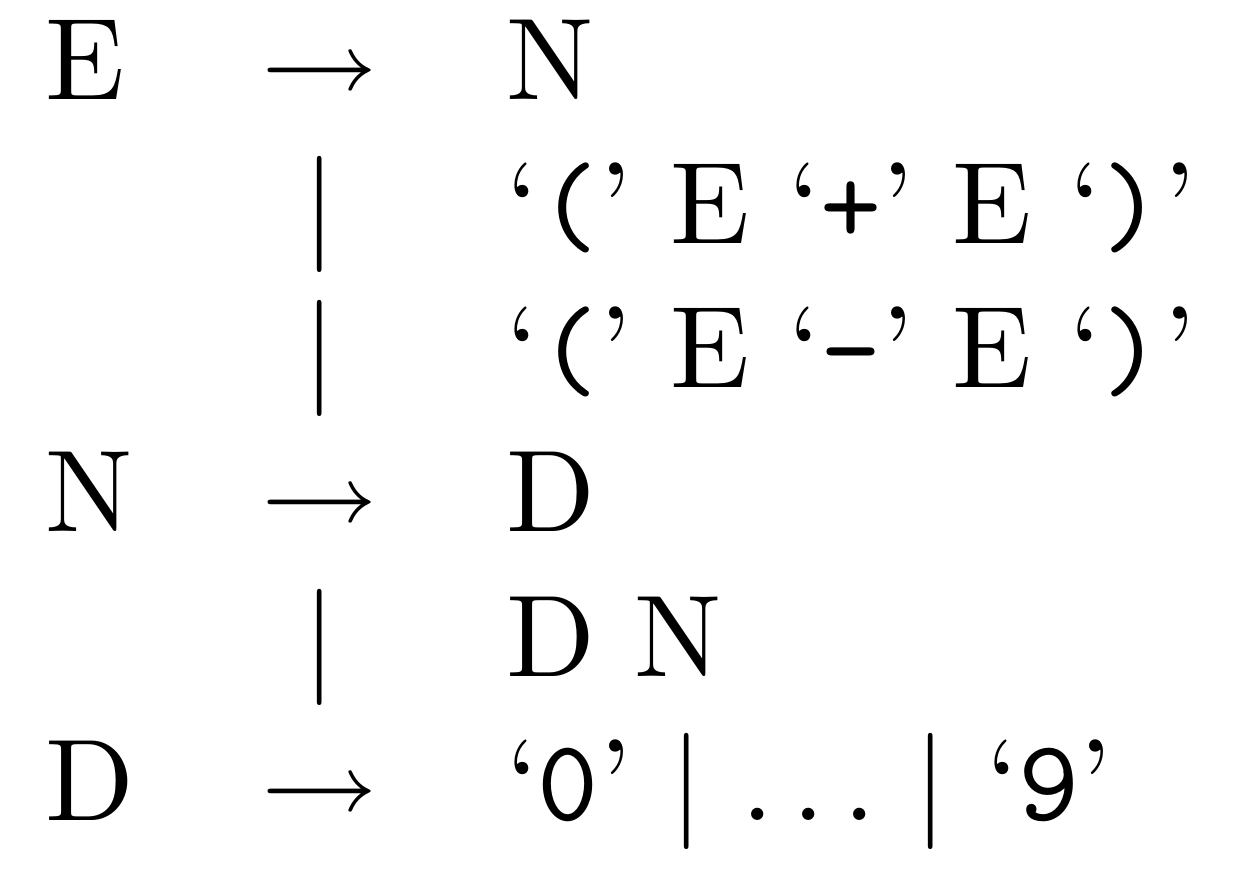
\includegraphics[width=0.3\textwidth]{pics/cfg_example}
    \caption{Μία CFG για μία απλή αριθμητική γλώσσα}
    \label{fig:cfg_example}
\end{figure}

Το Σχήμα \ref{fig:peg_example} παρουσιάζει την αντίστοιχη PEG.

\begin{figure}[h]
    \centering
    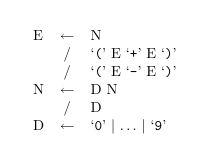
\includegraphics[width=0.3\textwidth]{pics/peg_example}
    \caption{Μία PEG για μία απλή αριθμητική γλώσσα}
    \label{fig:peg_example}
\end{figure}

Πρακτικά, η περιγραφή της γραμματικής μας ορίζει νοηματικά τί θα έκανε ένας καθοδικός συντακτικός αναλυτής για να αναγνωρίσει μία συμβολοσειρά στην είσοδο.

Το Σχήμα \ref{fig:peg_parse_example} απεικονίζει πώς η συμβολοσειρά `$(12-3)$' μπορεί να αναγνωριστεί σύμφωνα με τη γραμματική στο Σχήμα \ref{fig:peg_example} \cite{Ford2002a}.

\begin{figure}[h]
    \centering
    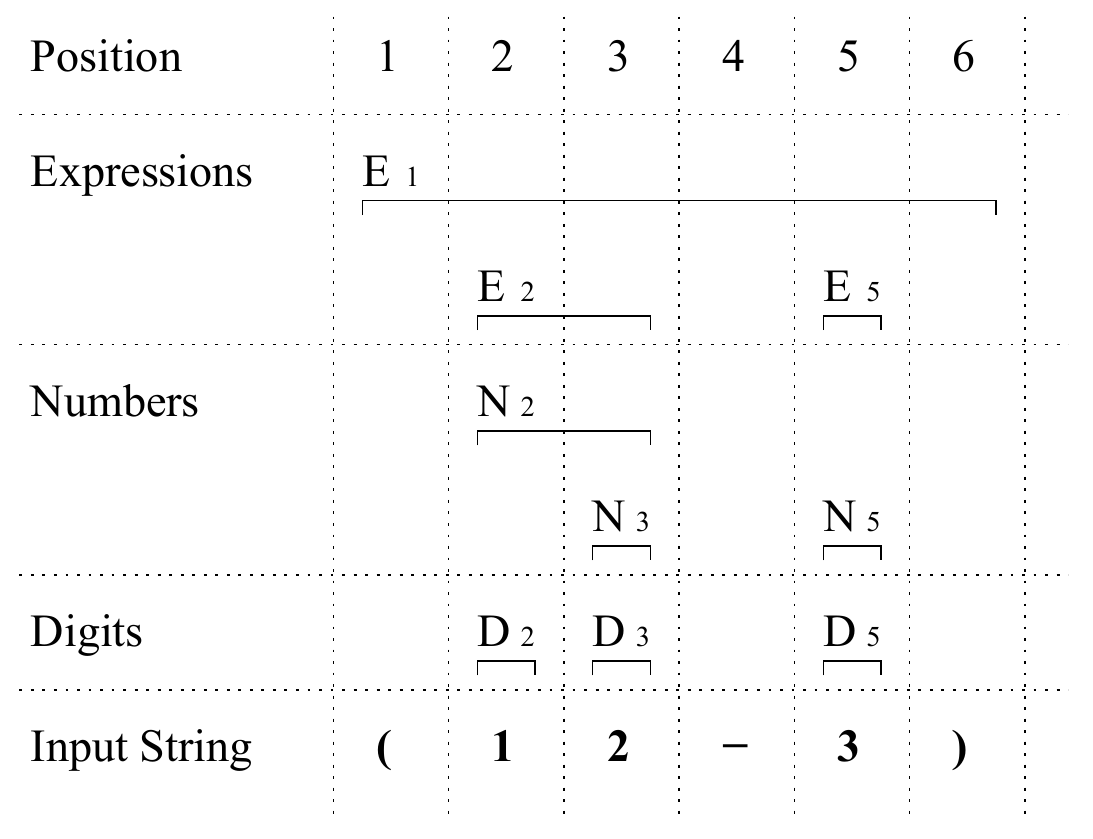
\includegraphics[width=0.5\textwidth]{pics/peg_parse_example}
	\caption{Αναγνωρίζοντας το `$(12-3)$' με βάση τη γραμματική στο Σχήμα \ref{fig:peg_example}}
    \label{fig:peg_parse_example}
\end{figure}

Ξεκινάμε προσπαθώντας να διαβάσουμε μία έκφραση $(E)$, από την αρχή της συμβολοσειράς.
Με βάση τον ορισμό της γραμματικής, για να αναγνωρίσει το μη τερματικό $E$, ο συντακτικός αναλυτής θα προσπαθούσε πρώτα να αναγνωρίσει την έκφραση $N$ που είναι η πρώτη εναλλακτική, οπότε προσπαθούμε και για τις δύο εναλλακτικές του $N$. Ωστόσο αποτυγχάνουμε καθώς στην είσοδο ο πρώτος χαρακτήρας είναι το '$($' και όχι κάποιο ψηφίο. 
Ακολούθως, πηγαίνουμε στη δεύτερη εναλλακτική για το $E$, τον κανόνα της πρόσθεσης εκφράσεων. 
Αυτός αναγνωρίζεται επιτυχώς με την αριστερή παρένθεση και μας καθοδηγεί στο να διαβάσουμε μία (υπο-)έκφραση ξεκινώντας στη θέση 2 της εισόδου.
Για να διαβάσουμε αυτή την υποέκφραση επιχειρούμε ξανά την $N$ εναλλακτική.
Πλέον, η πρώτη εναλλακτική του $N$ επιτυγχάνει, διαβάζοντας ένα ψηφίο στη θέση 2, και αναδρομικά ελέγχει για ένα ψηφίο στη θέση 3. 
Η πρώτη εναλλακτική του $N$ (δηλαδή η $D N$) αποτυγχάνει γιατί το ψηφίο στη θέση 3 δεν ακολουθείται από άλλα ψηφία, ωστόσο η δεύτερη εναλλακτική ($D$) επιτυγχάνει να αναγνωρίσει το ψηφίο, οπότε παράγει το αποτέλεσμα $N_3$ στο σχήμα. 
Η επιτυχημένη προσπάθεια καθιστά επιτυχημένη την αναγνώριση του $N$ στη θέση 2, οπότε το $N$ πλέον έχει ως αποτέλεσμα δύο κολλητούς χαρακτήρες, δηλαδή το $N_2$.
Αυτό οδηγεί στην έκφραση $E_2$ στο σχήμα. 
Επιστρέφοντας στο διάβασμα μίας έκφρασης στη θέση 1, η δεύτερη εναλλακτική αποτυγχάνει διότι η έκφραση $E_2$ ακολουθείται από ένα '$-$' αντί από ένα '$+$'.
Όμως, αν χρησιμοποιήσουμε την τρίτη εναλλακτική του $E$, αυτή επιτυγχάνει αφού αναγνωρίζει την αριστερή παρένθεση και την $E_2$ όπως και πριν, ενώ τώρα πετυχαίνει το '$-$', το ψηφίο $E_5$ στη θέση 5, και τη δεξιά παρένθεση. 
Επομένως, η έκφραση $E_1$ γεννιέται που αναγνωρίζει όλη τη συμβολοσειρά εισόδου.

\section{Άπληστη και Μη Ντετερμινιστική επανάληψη}
Ο κανόνας για το μη τερματικό $N$ δείχνει μία από τις πιο σημαντικές διαφορές μεταξύ των PEGs και των CFG γραμμτατικών.
Στη γραμματική του Σχήματος \ref{fig:cfg_example} η σειρά των δύο εναλλακτικών για το μη τερματικό δεν έχει σημασία, επειδή η επιλογή είναι μη ντετερμινιστική και προσανατολισμένη στο να γράφονται συμβολοσειρές και όχι να διαβάζονται.
Στην PEG του Σχήματος \ref{fig:peg_example}, η σειρά με την οποία εξετάζονται οι εναλλακτικές έχει σημασία: αν επιλέγαμε τη συντομότερη εναλλακτική πρώτα ($D$), τότε η μακρύτερη εναλλακτική δεν θα χρησιμοποιούνταν ποτέ.
Το αποτέλεσμα θα ήταν μία γραμματική που δεν θα μπορούσε να αναγνωρίσει τη συμβολοσειρά `$(12-3)$' διότι η ανάλυση του μη τερματικού στη θέση 2 θα κατανάλωνε μόνο το `$1$' στον αριθμό $12$, αφήνοντας το `$2$' να το αναγνωρίσουν άλλοι κανόνες ξεκινώντας πάλι από τη θέση 1.

Εξαιτίας αυτής της διαφοράς, οι δομές με επανάληψη σε μία PEG είναι εκ των πραγμάτων περισσότερο "άπληστες" παρά μη ντετερμινιστικές: μια επαναληπτική δομή πάντα καταναλώνει όσο περισσότερο κείμενο μπορεί, ανεξάρτητα από τα συμφραζόμενα στα οποία βρίσκεται. 
Αν στο παράδειγμά μας θέλαμε ξεφορτωθούμε το μη τερματικό $N$, θα μπορούσαμε να αντικαταστήσουμε την πρώτη εναλλακτική του $E$ με το `$D+$'.
Το αποτέλεσμα θα ήταν ακριβώς το ίδιο, γι' αυτό και ο τελεστής $+$ ονομάζεται "άπληστη θετική επανάληψη".

\section{Συντακτική ανάλυση ολόκληρων συμβολοσειρών}
Αν η γραμματική στο \ref{fig:peg_example} χρησιμοποιηθεί για να διαβάσει τη συμβολοσειρά `$(12-3)XYZ$', με αρχικό σύμβολο το $E$, τότε το αποτέλεσμα θα είναι "επιτυχία", ωστόσο μόνο το `$(12-3)$' θα έχει καταναλωθεί, αφήνοντας το `$XYZ$' ως υπόλοιπο. 
Όταν η πρόθεσή μας είναι να αναλύσουμε συντακτικά μία συμβολοσειρά, συνήθως θέλουμε να το κάνουμε μέχρι τέλους, και όχι μόνο σε ένα τμήμα της.
Ευτυχώς, η συμπεριφορά αυτή είναι εύκολο να υλοποιηθεί προσθέτοντας ένα νέο αρχικό σύμβολο $S$ όπως φαίνεται στο Σχήμα \ref{fig:whole_input}.

\begin{figure}[h]
    \centering
	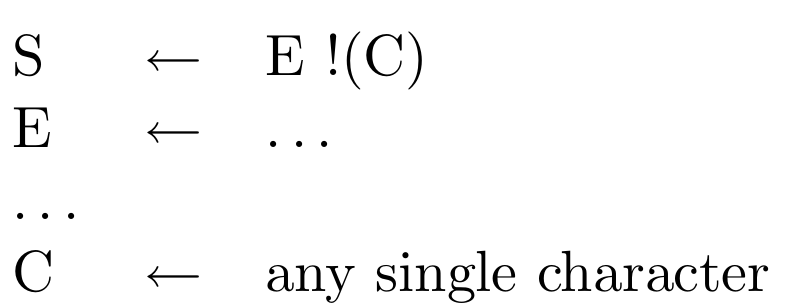
\includegraphics[width=0.4\textwidth]{pics/whole_input}
	\caption{Επέκταση της γραμματικής ώστε να εξετάζει όλη την είσοδο μέχρι τέλους}
    \label{fig:whole_input}
\end{figure}

Το αρχικό σύμβολο ψάχνει για μία έκφραση $E$, και μετά χρησιμοποιεί τον τελεστή "δεν-ακολουθείται-από" για να διασφαλίσει ότι τίποτα δεν έπεται μετά την αναγνωρισμένη έκφραση στην είσοδο.
Αν υπάρχει επιπλέον κείμενο που ακολουθεί την έκφραση, τότε το $C$ θα επιτύχει, κάνοντας το $S$ να αποτύχει. Αλλιώς, το $C$ αποτυγχάνει και το $S$ επιτυγχάνει.

Το $C$ σε αυτό το παράδειγμα είναι ένα μη τερματικό που αναπαριστά την \textit{κλάση χαρακτήρων}.

\section{Αριστερή Αναδρομή}

Σε μία γραμματική χωρίς συμφραζόμενα, τόσο η \textit{αριστερή} όσο και η \textit{δεξιά} αναδρομή επιτρέπονται. 
Ένα αριστερά αναδρομικό μη τερματικό έχει την ιδιότητα, αφού αναπτυχθεί μία ή περισσότερες φορές, να δίνει συμβολοσειρές η οποίες ξεκινούν με αυτό το μη τερματικό. 
Ομοίως, ένα δεξιά αναδρομικό μη τερματικό έχει την ιδιότητα να αναπτύσσεται σε συμβολοσειρές που \textit{τελειώνουν} με αυτό. 
Για παράδειγμα, είναι σύνηθες να εκφράζουμε τη σύνταξη αριστερά προσεταιριστικών τελεστών στα πλαίσια αριστερά αναδρομικών CFGs, και δεξιά προσεταιριστικούς τελεστές στα πλαίσια δεξιά αναδρομικών CFGs:

\begin{figure}[h]
    \centering
	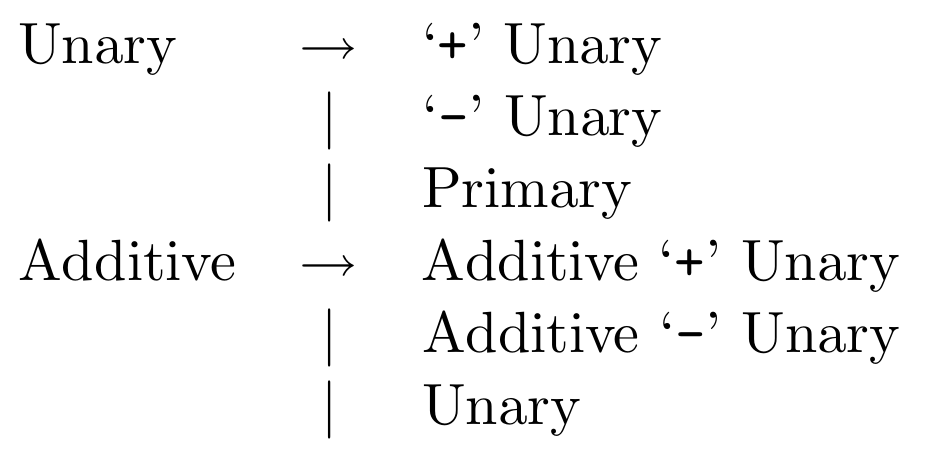
\includegraphics[width=0.45\textwidth]{pics/left_recursion}
	\caption{Αριστερά και δεξιά προσεταιριστικοί τελεστές σε μία CFG}
    \label{fig:left_recursion}
\end{figure}

Σε μία CFG ο δεξιά αναδρομικός ορισμός του $Unary$ υλοποιεί τους δεξιά προσεταιριστικούς μοναδιαίους τελεστές `$+$' και `$-$'.
Ομοίως, το $Additive$ υλοποιεί τους αριστερά προσεταιριστικούς τελεστές `$+$' και `$-$'.
Σε μία PEG, ενώ η δεξιά αναδρομή δουλεύει παρόμοια με τις CFGs, η αριστερή αναδρομή είναι εξ ορισμού λαθεμένη, καθώς η ερμηνεία της οδηγεί σε μία εκφυλισμένη αυτο-αναφορά. 
Για παράδειγμα, αν πάμε να εφαρμόσουμε αυτολεξεί τον κανόνα $Additive$ στα πλαίσια μίας PEG, τότε η ερμηνεία θα ήταν η εξής:
"Για να διαβάσεις μία $Additive$ έκφραση, πρώτα προσπάθησε να διαβάσεις μία $Additive$ έκφραση κ.ό.κ".

Σε μία CFG η αριστερή αναδρομή μπορεί να είναι βολική, ωστόσο δεν είναι απαραίτητη, καθώς οποιαδηποτε CFG που περιλαμβάνει αριστερή αναδρομή, μπορεί να γραφτεί σε μία ισοδύναμη CFG χωρίς αριστερή αναδρομή \cite{Moore2000}. 
Στις PEGs, συνήθως είναι πιο βολικό και ακριβές να χρησιμοποιούνται οι τελεστές `$*$' και `$+$', αντί της αριστερής ή της δεξιάς αναδρομής. 
Για παράδειγμα, η CFG του Σχήματος \ref{fig:left_recursion} μπορεί να γραφεί σε PEG ως:

\begin{figure}[h]
    \centering
	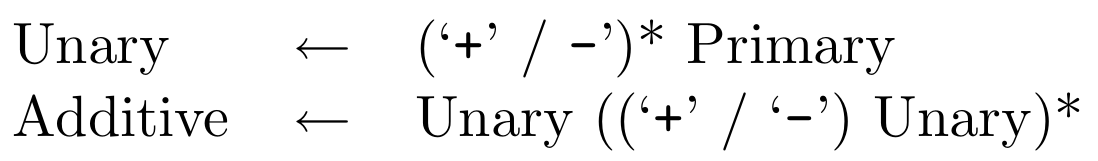
\includegraphics[width=0.45\textwidth]{pics/left_recursion_fix}
	\caption{Ισοδύναμη PEG χωρίς αριστερή αναδρομή}
    \label{fig:left_recursion_fix}
\end{figure}

Πάντως, αν είναι απαραίτητο, οι συντακτικοί αναλυτές των PEGs (τους οποίους θα περιγράψουμε παρακάτω), μπορούν να τροποποιηθούν ώστε να υποστηρίζουν αριστερή αναδρομή \cite{Warth2008}.

\chapter{ Packrat Parsing }

Το \textit{Packrat Parsing} \cite{Ford2002a} είναι μία τεχνική για την υλοποίηση συντακτικών αναλυτών για Parsing Expression Grammars.
Ένας συντακτικός αναλυτής packrat, ή αλλιώς packrat parser, προσφέρει την ισχύ και την ευελιξία ενός συντακτικού αναλυτή από πάνω προς τα κάτω με υπαναχώρηση (backtracking) και δυνατότητα ανάγνωσης άπειρων προπορευόμενων συμβόλων (infinite lookahead), αλλά εγγυάται γραμμικό χρόνο συντακτικής ανάλυσης.
Οποιαδήποτε γλώσσα ορισμένη από μία LL($k$) ή LR($k$) γραμματική μπορεί να αναγνωριστεί από έναν packrat parser, όπως και άλλες γλώσσες οι οποίες δεν υποστηρίζονται από συμβατικούς γραμμικούς αλγορίθμους.

Αυτή η επιπλέον ισχύς απλοποιεί τη διαχείριση των συνηθισμένων συντακτικών ιδιωμάτων όπως ο κανόνας της μακρύτερης αντιστοίχισης (longest-match rule), επιτρέπει τη χρήση συντακτικών και σημασιολογικών κατηγορημάτων για αποσαφήνιση (disambiguation), παρέχει καλύτερες ιδιότητες για σύνθεση γραμματικών (grammar composition), ενώ δίνει και τη δυνατότητα να ενσωματωθεί η λεκτική ανάλυση στη συντακτική.
Παρόλα αυτά, το packrat parsing θυμίζει την απλότητα και την κομψότητα συντακτικών αναλυτών αναδρομικής κατάβασης.

\section{Θεμέλια}

Ο απλούστερος και διαισθητικά προφανής τρόπος να σχεδιάσουμε έναν συντακτικό αναλυτή είναι η από πάνω προς τα κάτω ανάλυση ή ανάλυση αναδρομικής κατάβασης ή καθοδική συντακτική ανάλυση.
Σε αυτήν, τα στοιχεία της γλώσσας μεταφράζονται σχεδόν άμεσα σε ένα σύνολο από αμοιβαία αναδρομικές συναρτήσεις.
Η καθοδική συντακτική ανάλυση μπορεί να θεωρηθεί ως το πρόβλημα της κατασκευής ενός συντακτικού δέντρου για μια συμβολοσειρά εισόδου, ξεκινώντας από τη ρίζα και δημιουργώντας τους κόμβους του συντακτικού δε΄ντρου με πρωτοδιάταξη (preorder) \cite{Aho2006}. Ισοδύναμα, η καθοδική ανάλυση μπορεί να θεωρηθεί ως η εύρεση ενός αριστερότερου σχηματισμού παραγώγου για τη συμβολοσειρά εισόδου.

Οι καθοδικοί συντακτικοί αναλυτές μπορούν να διακριθούν σε δύο κατηγορίες. Οι \textit{προβλέποντες (predictive) συντακτικοί αναλυτές} επιχειρούν να προβλέψουν ποιοι στοιχείο της γλώσσας ακολουθεί βλέποντας ορισμένα από τα προβπορευόμενα σύμβολα στην είσδο.
Οι \textit{συντακτικοί αναλυτές με οπισθαναχώρηση (backtracking)} παίρνουν αποφάσεις υποθετικά (speculatively) και δοκιμάζουν διαδοχικά διάφορες εναλλακτικές: αν μία αποτύχει, τότε ο αναλυτής οπισθαναχωρεί στήν θέση της εισόδου πρωτού δοκιμάσει την εναλλακτική, και πάει στην επόμενη. 

Οι προβλέποντες συντακτικοί αναλυτές είναι γρήγοροι και εγγυώνται γραμμικό χρόνο στην ανάλυση (ως προς το μήκος της εισόδου), ενώ οι αναλυτές με οπισθαναχώρηση είναι πιο απλοί εννοιολογικά αλλά μπορεί να έχουν εκθετικό χρονο εκτέλεσης.

Το packrat parsing αποτελεί μία στρατηγική καθοδικής ανα΄λυσης που αξιοποιεί τα θετικά και από τις δύο πάνω επιλογές. 
Αφενός προσφέρει απλότητα, κομψότητα και γενικόττηα όπως ένας αναλυτής με οπισθαναχώρηση, αφετέρου εξοβελίζει τον εκθετικό χρόνο εκτέλεσης, αποθηκεύοντας ενδιάμεσα αποτελέσματα από τη συντακτική ανάλυση, ώστε κανένα αποτέλεσμα να μην υπολογιστεί παραπάνω από μία φορά.

Ένας packrat parser μπορεί εύκολα να κατασκευαστεί για οποιαδήποτε γλώσσασ που περιγράφεται από μία LL($k$) ή LR($k$) γραμματική, καθώς επίσης και για πολλές γλώσσες που απαιτούν infinite lookahead και δεν είναι, επομένως, LR.
Επιπλέον, είναι πιο εύκολο να κατασκευαστεί από έναν LR αναλυτή (ανοδική ανάλυση), ακόμα και με το χέρι.

\section{Υλοποιήση ενός packrat parser}

\subsection{Υλοποίηση της γραμματικής}
Το packrat parsing είναι θεμελιωδώς μία στρατηγική καθοδικής συντακτικής ανάλυσης, οπότε η υλοποίησή του σχετίζεται στενά με τους αναλυτές αναδρομικής κατάβασης. 
Θεμελιώδη ρόλο στην υλοποίηση και στους μετέπειτα πειραματισμούς μας παίζει και ο τρόπος με τον οποίο θα μοντελοποιήσουμε τον αναλυτή αλλά και όλη τη διαδικασία της ανάλυσης, ώστε να αποτυπωθούν σε κώδικα. 
Σε μία γλώσσα αντικειμενοστραφούς προγραμματισμού, όπως η C++, ένας τέτοιος αναλυτής θα μπορούσε να αναπαρασταθεί με ένα αντικείμενο. Το ίδιο και τα διάφορα επιμέρους κομμάτια που αποτελούν την εκάστοτε γραμματική. 

Για καλύτερη οπτικοποίηση και κατανόηση, παραθέτουμε τα UML διαγράμματα που απεικονίζουν την αναπαράσταση όσων περιγράψαμε στη θεωρία που προηγήθηκε. Θεωρούμε ότι τα διαγράμματα παρουσιάζουν μια απλοποιημένη C++ σύνταξη.

\begin{figure}[h]
    \centering
	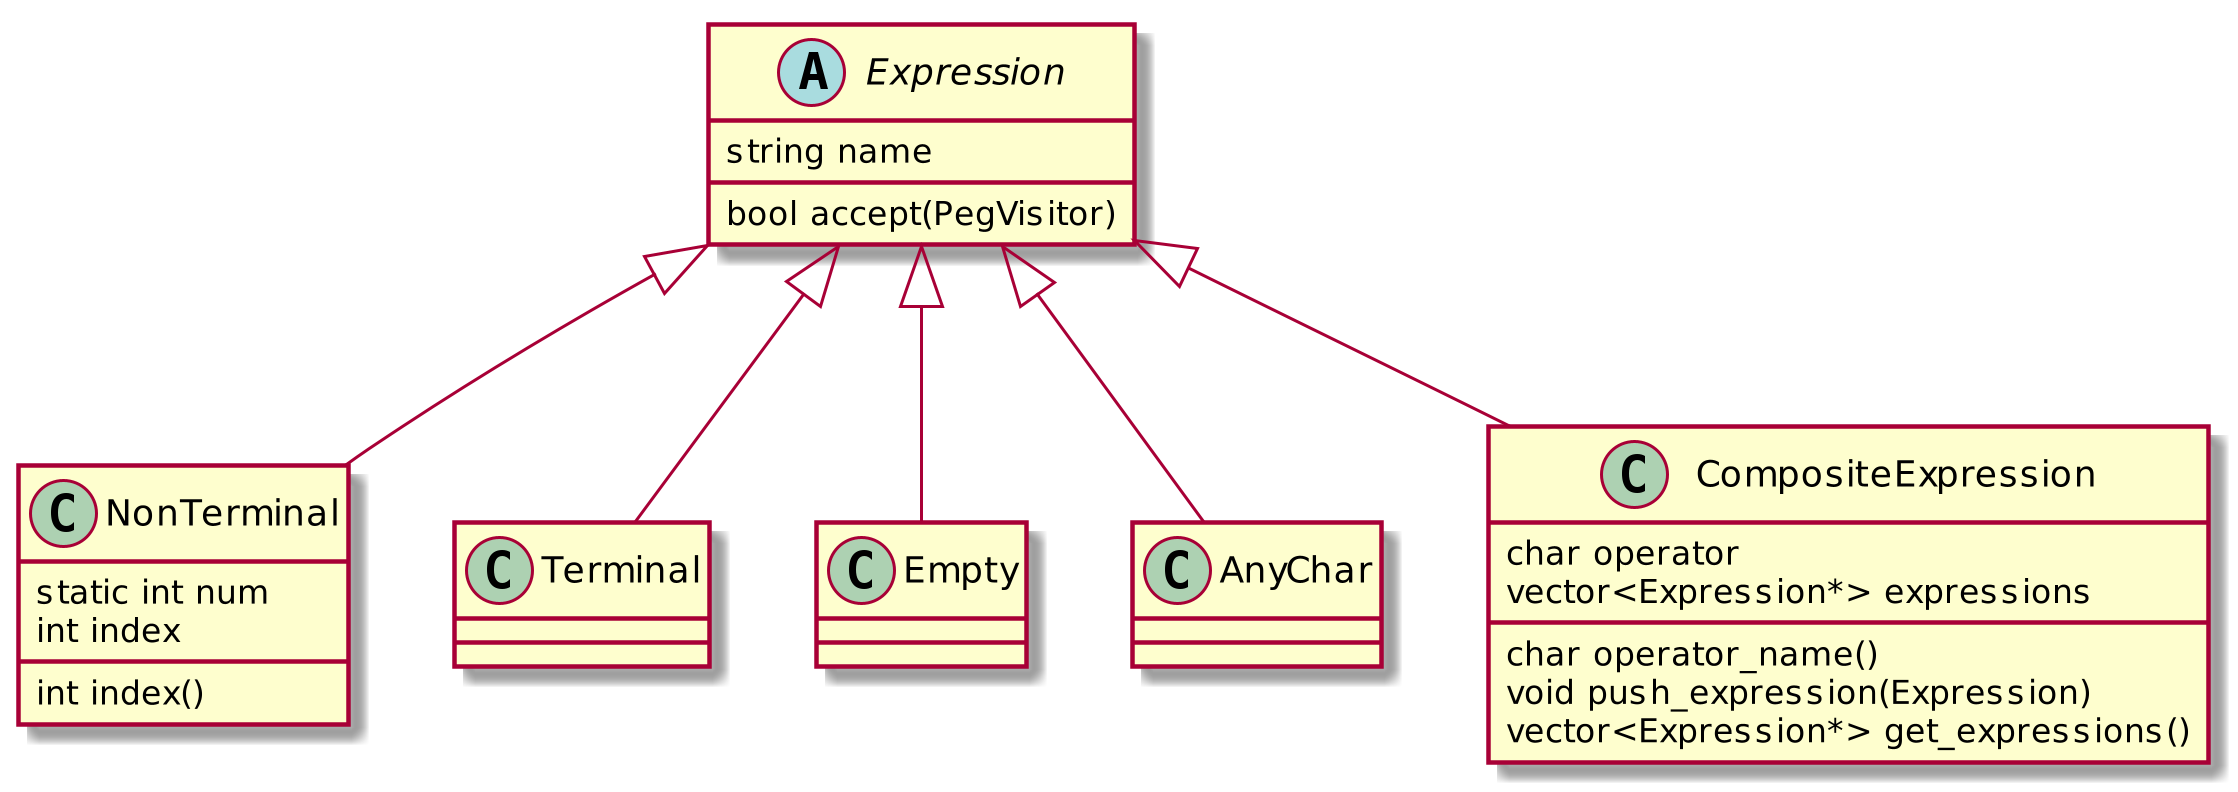
\includegraphics[width=1.10\textwidth]{uml/peg_elements}
	\caption{Μοντελοποίηση των δομικών στοιχείων μίας PEG}
    \label{fig:peg_elements}
\end{figure}

Όλες οι δομικές μονάδες της γραμματικής (τερματικά, μη τερματικά και οι σύνθετες εκφράσεις που τα περιέχουν) είναι εκφράσεις. 
Έτσι, προκύπτουν οι κλάσεις NonTerminal, Terminal και CompositeExpression που κληρονομούν την αφηρημένη κλάση Expression.
Επιπλέον χρειαζόμαστε και μία έκφραρση που να αναπαριστά τγην κενή συμβολοσειρά (Empty), καθώς και μία μου να αναπαριστά οποιονδήποτε χαρακτήρα (AnyChar).
Κατ' ελάχιστο, όλες οι εκφράσεις πρέπει να έχουν ένα όνομα, καθώς και να "δέχονται" έναν "επισκέπτη" (visitor pattern).
Όπως θα δούμε, ο επισκέπτης αυτός είναι ο συντακτικός αναλυτής που θα προσπαθήσει να τις αναγνωρίσει.

Επιπλέον, κάθε μη τερματικό θεωρούμε ότι αντιστοιχεί σε έναν μοναδικό ακέραιο index. 
Ακόμη, το CompositeExpression θεωρούμε ότι αποτελεί το σύνολο των Expressions που συνδέονται με έναν μόνο τελεστή.Για παράδειγμα:

\begin{equation}
	A / (B C)
\end{equation}

Εδώ υπάρχει ένα CompositExpression (έστω $C_1$) με τελεστή την ακολουθία και εκφράσεις τα $B$ και $C$, καθώς και ένα CompositeExpression με τελεστή την διατεταγμένη επιλογή (`$/$') και εκφράσεις τα $A$ και $C_1$. 
Στο διάγραμμα φαίνονται ενδεικτικά οι βασικές μέθοδοι των κλάσεων με βάση τα πεδία που περιγράψαμε.

Με βάση αυτές τις δομικές μονάδες κατασκευάζουμε την κλάση μίας γραμματικής PEG, όπως φαινεται στο Σχήμα \ref{fig:peg}.

\begin{figure}[h]
    \centering
	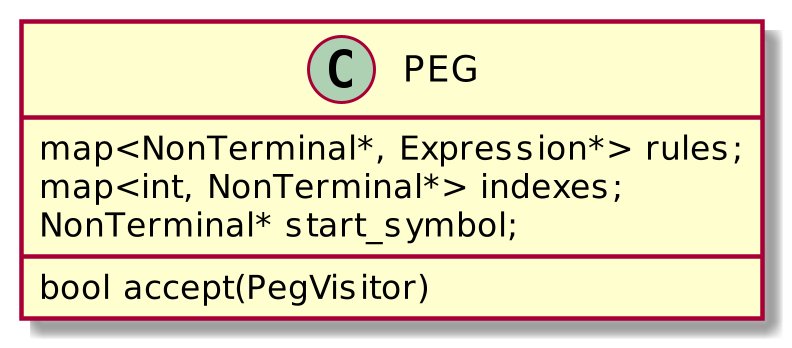
\includegraphics[width=0.50\textwidth]{uml/peg}
	\caption{Μοντελοποίηση μίας PEG}
    \label{fig:peg}
\end{figure}

\begin{minipage}{\textwidth}

Επομένως, τα βασικά πεδία μίας PEG είναι τα εξής:

\begin{description}[font=$\bullet$\scshape\bfseries]
	\item rules: Οι κανόνες θεωρούμε ότι είναι μία αντιστοίχιση από μη τερματικά σε σύνθετες εκφράσεις
	\item indexes: Η γραμματική ενσωματώνει την πληροφορία για την αντιστοιχία των μη τερματικών με μοναδικούς ακεραίους.
	\item start\_symbol: Το αρχικό σύμβολο της γραμματικής
\end{description}

\end{minipage}

\subsection{Υλοποίηση του συντακτικού αναλυτή}

Αφού μοντελοποιήσαμε μία PEG, μπορούμε τώρα να κάνουμε το ίδιο και για έναν συντακτικό αναλυτή για αυτήν. 
Είπαμε ότι το Packrat Parsing συνδύαζει τα πλεονεκτήματα της απλότητας του αναλυτή αναδρομικής κατάβασης με οπισθαναχώρηση και της ταχύτητας του προβλέποντα συντακτικού αναλυτή. 
Αυτό το πετυχαίνει κρατώντας τα ενδιάμεσα αποτελέσματα που υπολογίζει σε έναν \textit{πίνακα υπομνηματισμού (memoisation table)}.

Ο πίνακας αυτός έχει σειρές που αντιστοιχούν σε ένα μη τερματικό της γραμματικής και στήλες που αντιστοιχούν σε μία συγκεκριμένη θέση στην είσοδο. Έτσι, το κελί $(i, j)$ περιέχει το αποτέλεσμα που θα πάρουμε αν προσπαθήσουμε με το μη τερματικό $i$ να αναγνωρίσουμε το κομμάτι της εισόδου από τη θέση $j$ και μετά. 
Αυτόν τον πίνακα, μπορούμε είτε να τον γεμίσουμε από πάνω προς τα κάτω, δηλαδή κάνοντας αναδρομική κατάβαση με υπομνηματισμό (memoisation), είτε από κάτω προς τα πάνω, στο πνεύμα του δυναμικού προγραμματισμού.

Στην εκδοχή του δυναμικού προγραμματισμού ξεκινάμε να γεμίζουμε τα κελιά από το δεξί άκρο της εισόδου προς τα αριστερά, και κινούμαστε από τα κατώτερα κελιά στα ανώτερα μέσα σε κάθε στήλη. 
Οποτεδήποτε συμπληρώνουμε ένα κελί το αποτέλεσμά του αποθηκεύεται και μπορεί να χρησιμοποιηθεί έτοιμο στις κλήσεις άλλων κελιών που δεν έχουν υπολογιστεί ακόμα.

Έστω η ακόλουθη γραμματική:

\begin{figure}
	\begin{equation}
		\begin{array}{l}
			Additive \; \leftarrow \; Multitive \; \mlq + \mrq \; Additive \; | \; Multitive \\
			Multitive \; \leftarrow \; Primary \; \mlq * \mrq \; Multitive \; | \; Primary \\
			Primary \; \leftarrow \; \mlq ( \mrq \; Additive \mlq \; ) \mrq \; | \; Decimal \\
			Decimal \; \leftarrow \; \mlq 0 \mrq \; | \; ... \; | \; \mlq 9 \mrq \; 
		\end{array}
	\end{equation}
\caption{Μία PEG γραμματική για αριθμητικές εκφράσεις}
\label{fig:peg_example_def}
\end{figure}

Ο Πίνακας \ref{tab:packrat_dp_example} παρουσιάζει έναν μερικώς συμπληρωμένο πίνακα για είσοδο τη συμβολοσειρά ${2 * (3 + 4)}$.

\begin{longtable}{lllllllll}
    column & C1 & C2& C3& C4& C5& C6& C7& C8 \\
    \hline
    Additive&  & & $\uparrow$& (7,C7)& X& (4,C7)& X& X \\
    Multitive& &  & \vdots & (3,C5)& X& (4,C7)& X& X \\
    Primary &   & $\leftarrow$ \ldots & \circled{?}& (3,C5)& X& (4,C7)& X& X \\
    Decimal &  & & X& (3,C5)& X& (4,C7)& X& X\\
    \hline
    Input String & '2'& '*' & '('& '3'& '+'& '4'& ')'& EOF\\
	\\

	\caption{Ενδιάμεσα αποτελέσματα  για την είσοδο ${2 * (3 + 4)}$}
    \label{tab:packrat_dp_example}
\end{longtable}

Κάθε στήλη $C_j$ αντιστοιχεί στο σημείο $j$ της εισόδου.
Κάθε γραμμή (pAdditive, pMultitive κλπ) αντιστοιχεί στη συνάρτηση που αναλύει συντακτικά το μη τερματικό $i$.
Για λόγους παρουσίασης κάθε κελί παρουσιάζεται με δύο τιμές (η υλοποίηση θα είχε διαφορετικές).
Η μία τιμή είναι η σημασιολογική τιμή που επιστρέφεται ως αποτέλεσμα της συντακτικής ανάλυσης.
Η άλλη είναι η στήλη στην οποία θα πάει μετά η ανάλυση, μόλις καταναλώσει μέρος της εισόδου σε εκείνο το κελί.

Για παράδειγμα, στη στήλη C4, στη γραμμή Additive, η ερμηνεία είναι η εξής: 
Αν η συνάρτηση που αντιστοιχεί στο Additive, ξεκινήσει την συντακτική ανάλυση από τη θέση 4 (χαρακτήρας `3'), θα καταναλώσει 3 χαρακτήρες (την παράσταση $3+4$) και θα φτάσει μέχρι το σημείο 7 της εισόδου. 
Η σημασιολογική τιμή που θα επιστραφεί είναι το αποτέλεσμα της έκφρασης, δηλαδή το 7.

Το επόμενο κελί που θα πρέπει να υπολογιστεί είναι το Primary στη στήλη C3.
Για να δείξουμε ένα παράδειγμα πώς επαναχρησιμοποιούνται τα αποτελέσματα, εστιάζουμε σε αυτό το κελί.

Ο κανόνας για το Primary έχει δύο εναλλακτικές: 
μία έκφραση για το Additive με παρενθέσεις ή ένα Decimal.
Αν προσπαθήσουμε τις εναλλακτικές με τη σειρά που δίνεται στη γραμματική, το Primary πρώτα θα ελέγξει για Additive ανάμεσα σε παρενθέσεις.
Για να γίνει αυτό, πρώτα αντιστοιχίζει την αριστερή παρένθεση στη στήλη C3, το οποίο πετυχαίνει και επιστρέφει την υπόλοιπη συμβολοσειρά η οποία ξεκινάει στη στήλη C4, δηλαδή την $`3+4)'$.
Στην έκδοση του αναλυτή αναδρομικής κατάβασης με οπισθαναχώρηση, το Primary θα έπρεπε να καλέσει αναδρομικά τη συνάρτηση Additive στην εναπομείνασα συμβολοσειρά. 
Ωστόσο, επειδή έχουμε αποθηκεύσει τα ενδιάμεσα αποτελέσματα στον πίνακα,μπορούμε απλά να κοιτάξουμε το αποτέλεσμα της κλ΄σης Additive στη στήλη C4, που είναι (7,C7). 
Οπότε, η σημασιολογική τιμή είναι το 7 και η νέα θέση που εξετάζουμε στη συμβολοσειρά ξεκινάει στη στήλη C7, όπου βρίσκεται η δεξιά παρένθεση.
Εφόσον, η υποέκφραση της γραμματικής έχει και αυτή το μη τερματικό `)', ο κανόνας πετυχαίνει στη θέση C7, καταναλώνει την παρένθεση και αφήνει το υπόλοιπο στη θέση C8.
Τελικά, το αποτέλεσμα για το Primary στη θέση C3 είναι (7, C8).

Το μέγεθος του πίνακα μεγαλώνει με το μήκος της συμβολοσειράς εισόδου αλλά μόνο γραμμικά, υποθέτοντας ότι η γραμμτική έχει πεπερασμένο αριθμό από μη τερματικά σύμβολα.
Επιπλέον, θεωρώντας ότι η γραμματική είναι εκφρασμένη σε Backus-Naur Normal Form, μόνο ένας συγκεκριμένος αριθμός από ενδιάμεσα αποτελέσματα χρειάζεται να προσπελαστεί για να υπολογιστεί ένα νέο αποτέλεσμα.
Επομένως, υποθέτοντας ότι η προσπέλαση ενός κελιού παίρνει σταθερό χρόνο (π.χ. για υλοποίηση με δισδιάστατο πίνακα), η όλη διαδικασία είναι γραμμική ως προς το μήκος της εισόδου.

Ακριβώς επειδή κάθε κελί έχει έναν "δείκτη" προς την επόμενη θέση της εισόδου που θα συνεχιστεί η συντακτική ανάλυση, μπορεί να συμβουλευτεί κελιά που βρίσκονται αυθαίρετα μακριά στον πίνακα.
Για παράδειγμα, ο υπολογισμός του κελιού [Primary, C3] χρειάστηκε αποτελέσματα από τις στήλες C3, C4 και C7. 
Αυτή η ικανότητα να προσπερνάει προπορευόμενα σύμβολα στην είσοδο είναι που του δίνει το infinite lookahead και τον κάνει πιο ισχυρό από έναν LR αναλυτή γραμμικού χρόνου.

Ένα προφανές πρακτικό πρόβλημα της προσέγγισης με το δυναμικό προγραμμτισμό, όπου τα κελιά υπολογίζονται όλα από δεξιά προς τα αριστερά και από κάτω προς τα πάνω, είναι ο υπολογισμός πολλών ενδιάμεσων αποτελεσμάτων που δεν θα χρειαστούν. 
Μία επιπλέον δυσχέρεια είναι πως πρέπει εκ των προτέρων να καθορίσουμε τη σειρά με την οποία θα υπολογιστούν τα κελιά μιας στήλης.
Εμείς είπαμε ότι υπολογίζονται από κάτω προς τα πάνω, όμως αυτό προϋποθέτει εξ αρχής να έχουμε βάλει τη σειρά των μη τερματικών με τέτοιο τρόπο ώστε τα κάτω κελιά που υπολογίζονται πρώτα, να μην εξαρτώνται από τα πάνω.
Για παράδειγμα, στο Σχήμα \ref{fig:peg_example_def}, οι κανόνες παρουσιάζουν εξάρτηση από πάνω προς τα κάτω.

To Packrat Parsing είναι πρακτικά ένας αναδρομικός αλγόριθμος με υπομνηματισμό που λύνει και τα δύο προβλήματα.
Ένας packrat parser υπολογίζει αποτελέσματα μόνο όταν χρειάζονται, με την ίδια σειρά που θα ακολουθούσε και ένας αναλυτής αναδρομικής κατάβασης με οπισθαναχώρηση.
Όμως, άπαξ και ένα ενδιάμεσο αποτέλεσμα υπολογιστεί, αποθηκεύεται για μελλοντική χρήση.

Το Σχήμα παρουσι΄άζει τη δομή δεδομένων πυο δημιουργείται μετά από packrat parsing στην είσοδο $`2 * (3 + 4)'$, χρησιμοπιοώντας μία εννοιλογική αναπαράσταση με δείκτες που αναπαριστούν τη σχέση μεταξύ των κελιών.
Τα γκρίζα κουτιά δεν θα υπολογιστούν καθόλου.
Τα λευκά κουτιά που είναι διαγραμμένα δείχνουν αποτυχία συντακτικής ανάλυσης. 

Η αναπαράσταση καθιστά σαφές γιατί ο αλγόριθμος είναι πολυπλοκότητας $O(n)$ ως προς το μήκος $n$ της εισόδου.
Η πρώτη συνάρτηση είναι αυτή η οποία ξεκινά τις αναδρομικές κλήσεις προς άλλες συναρτήσεις.
Κάθε κελί υπολογίζεται το πολύ μία φορά, οπότε ο αλγόριθμος είναι γραμμικός ως προς την είσοδο. 
Προφανώς, η σειρά με την οποία υπολογίζονται τα ενδιάμεσα αποτελέσματα διαφέρει από τον προηγούμενο αλγόριθμο δυναμικού προγραμματισμού, που αναφέραμε νωρίτερα.

Πώς όμως θα μοντελοποιήσουμε έναν τέτοιο συντακτικό αναλυτή?
Είπαμε προηγουμένως ότι μία γραμματική PEG θα δέχεται έναν τέτοιον αναλυτή ως επισκέπτη (visitor).
Επιπλέον, ο parser μας πρέπει να ενθυλακώσει (encapsulate):

\begin{description}[font=$\bullet$\scshape\bfseries]
	\item: Τη συμβολοσειρά εισόδου
	\item: Τη συμβολοσειρά εισόδου

την πληροφορία της εισόδου που θα αναλύσει, τη δομή δεδομένων για τον πίνακα που θα αποθηκεύει τα ενδιάμεσα αποτελέσματα (

\section{Πλεονεκτήματα και Μειονεκτήματα}

\chapter{ Παράλληλο Packrat Parsing με Υπομνηματισμό }

\chapter{ Seith Fowler}

\chapter{ Παράλληλο Ordered Choice }

\chapter{ Παράλληλo Elastic Packrat Parsing }

\chapter{  Πειραματικά Αποτελέσματα }

\chapter{ Συμπεράσματα - Μελλοντική Δουλειά }

\englishtext

\chapter{Introduction}

\section{The Goal of this Project}

\section{The C++ Programming Language}


\begin{figure}[t]
\setlength\partopsep{-\topsep}% adjusts vertical space after the listing
\begin{minted}[frame=lines,linenos,numbersep=5pt]{c++}
#include <iostream>
int main() {
  std::cout << "Hello world!" << std::endl;
}
\end{minted}
\caption{Filled with joy, the Agha decides to write some code.%
  \label{fig:hello-english}}
\end{figure}


\section{The Structure of this Thesis}

\chapter{Theoretical Background}

\section{Programming Language Semantics}

\section{Domain Theory}

\selectlanguage{greek}


%%%  Bibliography

% You shouldn't want to include all the contents of thesis.bib
% in your bibliography (do you?)
\nocite{*}

\bibliographystyle{softlab-thesis}
\bibliography{thesis}


%%%  Appendices

\backmatter

\appendix

\chapter{Ευρετήριο συμβολισμών}

$A \rightarrow B$ : συνάρτηση από το πεδίο $A$ στο πεδίο $B$.

\chapter{Ευρετήριο γλωσσών}

\begin{description}
\item[C++:] πώς θα βγάλω λεφτά...
\item[Haskell:] η γλώσσα της ζωής μου αλλά πάνε οι μπύρες...
\item[Javascript:] χα, χα, χα...
\item[Python:] πώς θα τελειώνω για να πάω για μπύρες...
\end{description}


\chapter{Ευρετήριο αριθμών}

\begin{description}
\item[17:] ask Zachos.
\item[42:] life, the universe and everything --- ask Douglas.
\end{description}


%%%  End of document

\end{document}
